\documentclass[letterpaper, 10pt]{article}

\usepackage{amsfonts}
\usepackage{amsmath}
\usepackage{hyperref}
\usepackage{xcolor}
\usepackage[UTF8]{ctex}
\usepackage{geometry}
\usepackage{fontspec}
\usepackage{graphicx}
\usepackage{subfigure}

\geometry{left=2cm,right=2cm,top=2cm,bottom=2cm}
\hypersetup{
	colorlinks, linkcolor=blue, anchorcolor=blue, citecolor=blue
}

\newcommand{\qbar}{\rangle}
\newcommand{\qket}{\langle}
\newcommand{\dd}{\mathrm{d}}
\newcommand{\dbar}{\mathrm{d}\hspace*{-0.18em}\bar{}\hspace*{0.2em}}

\begin{document}

\title{热统习题的部分答案}
\author{}
\date{\today}
\maketitle
\thispagestyle{empty}

\tableofcontents

\newpage
\setcounter{page}{1}


\section[第一章]{第一章}

\subsection{习题1.6}
\begin{eqnarray*}
\alpha = \frac{1}{V} \left( \frac{\partial V}{\partial T} \right)_{p} = \frac{\nu R}{pV} & \Rightarrow & \left( \frac{\partial V}{\partial T} \right)_{p} = \frac{\nu R}{p} \\
& \Rightarrow & V = \frac{\nu R T}{p} + g(p) \quad{} \text{代入$ \kappa = \frac{1}{p} + \frac{a}{V} = - \frac{1}{V} \left( \frac{\partial V}{\partial p} \right)_{T} $} \\
& \Rightarrow & \dd( p g(p) ) = - \frac{a}{2} \dd ( p^2 ) \\
& \Rightarrow & p g(p) = - \frac{a}{2} p^2 + \mathrm{const} \quad{} \text{代入第二行式子并整理} \\
& \Rightarrow & pV = \nu RT - \frac{a}{2} p^2 + \mathrm{const}.
\end{eqnarray*}

\subsection{习题1.8}
\begin{itemize}
	\item[1)]
	利用广延量假设,
	\begin{eqnarray*}
	S = Ns, V = Nv, U = Nu & \Rightarrow & s = A(vu)^{1/3} \\
	&\Rightarrow & T \dd s = T A \frac{v \dd u + u \dd v}{3(vu)^{2/3}} = \dd u + p \dd v \\
	\text{$\dd u, \dd v$前的系数对应相等并恢复广延量} & \Rightarrow & 		 	
		\begin{cases}
		T = \frac{3u^{2/3}}{Av^{1/3}} = \frac{3U^{2/3}}{A(NV)^{1/3}} \quad{} \text{易得: $ U \sim T^{3/2} $} \\
		p = \left( \frac{N}{V} \right)^{1/2} \left( \frac{AT}{3} \right)^{3/2}
		\end{cases} \\
	\end{eqnarray*}
	\[ C_{V} = \left( \frac{\partial U}{\partial T} \right)_{V} = \frac{1}{2} \sqrt{\frac{A^3 NVT}{3}} \quad{} \text{利用了前面的温度表达式.} \]
	\item[2)]
	对于每个热源而言, 我们有: 
	\[ \dbar Q = \dd U \sim T^{1/2} \dd T, \]
	由于高温热源放出热量($ \Delta Q_{h} < 0 $)必定大于等于低温热源吸热($ \Delta Q_{c} > 0 $), 不失一般性, 我们假设$ T_{1} > T_{2} $, 
	\begin{eqnarray*}
	\Delta Q_{h} + \Delta Q_{c} \leq 0 & \Rightarrow & \left( \int_{T_{1}}^{T_{f}} + \int_{T_{2}}^{T_{f}} \right) T^{1/2} \dd T \leq 0 \\
	& \Rightarrow & T_{f} \leq \left( \frac{T_{1}^{3/2} + T_{2}^{3/2}}{2} \right)^{2/3};
	\end{eqnarray*}
	另一方面, 由热力学第二定律: $ \Delta S \geq 0 $,
	\begin{eqnarray*}
	\Delta S = \left( \int_{T_{1}}^{T_{f}} + \int_{T_{2}}^{T_{f}} \right) \frac{\dbar Q}{T} 
	\sim \left( \int_{T_{1}}^{T_{f}} + \int_{T_{2}}^{T_{f}} \right) \frac{1}{T^{1/2}} \dd T \geq 0 \\
	\Rightarrow \quad{} T_{f} \geq \left( \frac{T_{1}^{1/2}+T_{2}^{1/2}}{2} \right)^{2}.
	\end{eqnarray*}
	由第一题的温度表达式, 我们得到: 
	\[ U = \left( \frac{AT(NV)^{1/3}}{3} \right)^{3/2} = C T^{3/2}. \]
	对于整个系统而言,
	\[ W = - \Delta U_{\text{总}} = C \left( T_{1}^{3/2} + T_{2}^{3/2} - 2 T_{f}^{3/2} \right) \leq \sqrt{\frac{A^{3}NV}{27}} 
	\left[ T_{1}^{3/2} + T_{2}^{3/2} - 2 \left( \frac{T_{1}^{1/2}+T_{2}^{1/2}}{2} \right)^3 \right]. \]
\end{itemize}

\subsection{习题1.11}
首先,我们需要求出范氏气体的内能表达式, 
\begin{eqnarray*}
\text{由范氏气体的状态方程} & \Rightarrow & \left( \frac{\partial p}{\partial T} \right)_{V} = \frac{R}{V-b} \\
\text{代入书上式子($ 1.9.16 $)} & \Rightarrow & 
\left( \frac{\partial U}{\partial V} \right)_{T} = - p + T \left( \frac{\partial p}{\partial T} \right)_{V} = \frac{a}{V^{2}} \\
& \Rightarrow & \dd U = C_{V} \dd T + \left( \frac{\partial U}{\partial V} \right)_{T} \dd V = C_{V} \dd T + \frac{a}{V^{2}} \dd V \\
& \Rightarrow & U = C_{V} T - \frac{a}{V} + U_{0}.
\end{eqnarray*}
\begin{itemize}
	\item[1)]
	对于等温过程,
	\begin{align*}
	& \Delta U = - \frac{a}{V_{f}} + \frac{a}{V_{i}} \\
	& W = \int_{V_{i}}^{V_{f}} p \dd V = \int_{V_{i}}^{V_{f}} \left( \frac{RT_{i}}{V-b} - \frac{a}{V^2} \right) \dd V = 
	RT_{i} \ln \left( \frac{V_{f}-b}{V_{i}-b} \right) + \frac{a}{V_{f}} - \frac{a}{V_{i}} \\
	& \Delta S = \frac{\Delta U + W}{T_{i}} = R \ln \frac{V_{f}-b}{V_{i}-b};
	\end{align*}
	\item[2)]
	对于等压过程, 
	\[ W = p_{i} (V_{f} - V_{i}) = \left( \frac{RT_{i}}{V_{i}-b} - \frac{a}{V_{i}^2} \right) (V_{f} - V_{i}) \]
	\begin{eqnarray*}
	\text{利用状态方程} & \Rightarrow & T_{f} = \left( p_{i} + \frac{a}{V_{f}^2} \right)(V_{f} - b)/R = 
	\left( \frac{RT_{i}}{V_{i}-b} - \frac{a}{V_{i}^2} + \frac{a}{V_{f}^2} \right)(V_{f} - b)/R \\
	& \Rightarrow & \Delta U = C_{V}(T_{f} - T_{i}) - \frac{a}{V_{f}} + \frac{a}{V_{i}} = 
	C_{V}\left[ \left( \frac{RT_{i}}{V_{i}-b} - \frac{a}{V_{i}^2} + \frac{a}{V_{f}^2} \right)(V_{f} - b)/R - T_{i} \right] - \frac{a}{V_{f}} + \frac{a}{V_{i}}
	\end{eqnarray*}
	\begin{eqnarray*}
	\text{由等压条件} & \Rightarrow & T \dd S = \dbar Q = C_{p} \dd T \\
	& \Rightarrow & \dd S = C_{p} \dd(\ln T) \\
	& \Rightarrow & \Delta S = C_{p} \ln \frac{T_{f}}{T_{i}} = C_{p} \ln 
	\left[ \frac{V_{f}-b}{V_{i}-b} - a\left( \frac{1}{V_{i}^2} - \frac{1}{V_{f}^2} \right) \frac{V_{f}-b}{RT_{i}} \right];
	\end{eqnarray*}
	\item[3)]
	对于绝热过程, 
	\[ \dbar Q = \dd U + p \dd V = \left( \frac{\partial U}{\partial T} \right)_{V} \dd T + 
	\left[ \left( \frac{\partial U}{\partial V} \right)_{T} + p \right] \dd V = C_{V} \dd T + \left( \frac{a}{V^{2}} + p \right) \dd V = 0, \]
	\begin{eqnarray*}
	\text{结合状态方程} & \Rightarrow & C_{V} \dd T + \frac{RT}{V-b} \dd V = 0 \\
	& \Rightarrow & C_{V} \ln T + R \ln (V-b) = 0 \\
	& \Rightarrow & T^{C_{V}} (V-b)^{R} = \mathrm{const} \\
	& \Rightarrow & T_{f} = T_{i} \left( \frac{V_{i}-b}{V_{f}-b} \right)^{R/C_{V}}
	\end{eqnarray*}
	因此, 我们容易得到:
	\begin{align*}
	& \Delta U = C_{V} T_{i} \left[ \left( \frac{V_{i}-b}{V_{f}-b} \right)^{R/C_{V}} - 1 \right] - \frac{a}{V_{f}} + \frac{a}{V_{i}} \\
	& W = - \Delta U \\
	& \Delta S = 0.
	\end{align*}
\end{itemize}

\subsection{习题1.13}
其中一个物体降温(放热): $ T_{1} \rightarrow T_{2} $, 另一个物体升温(吸热): $ T_{1} \rightarrow T_x $. 考虑整个体系, 由热力学第二定律, 
\[ \Delta S = \left( \int_{T_{1}}^{T_{2}} + \int_{T_{1}}^{T_x} \right) \frac{C_{p}\dd T}{T} \geq 0 \quad{} \Rightarrow \quad{} T_x \geq \frac{T_{1}^2}{T_{2}}. \]
因此, 
\[ W \geq \Delta U = C_{p} (T_x + T_{2} - 2T_{1}) \geq C_{p} \left( \frac{T_{1}^2}{T_{2}} + T_{2} - 2 T_{1} \right) = C_{p} \frac{(T_{1}-T_{2})^2}{T_{2}}. \]

\subsection{习题1.22}
\begin{figure}[htbp]
\centering
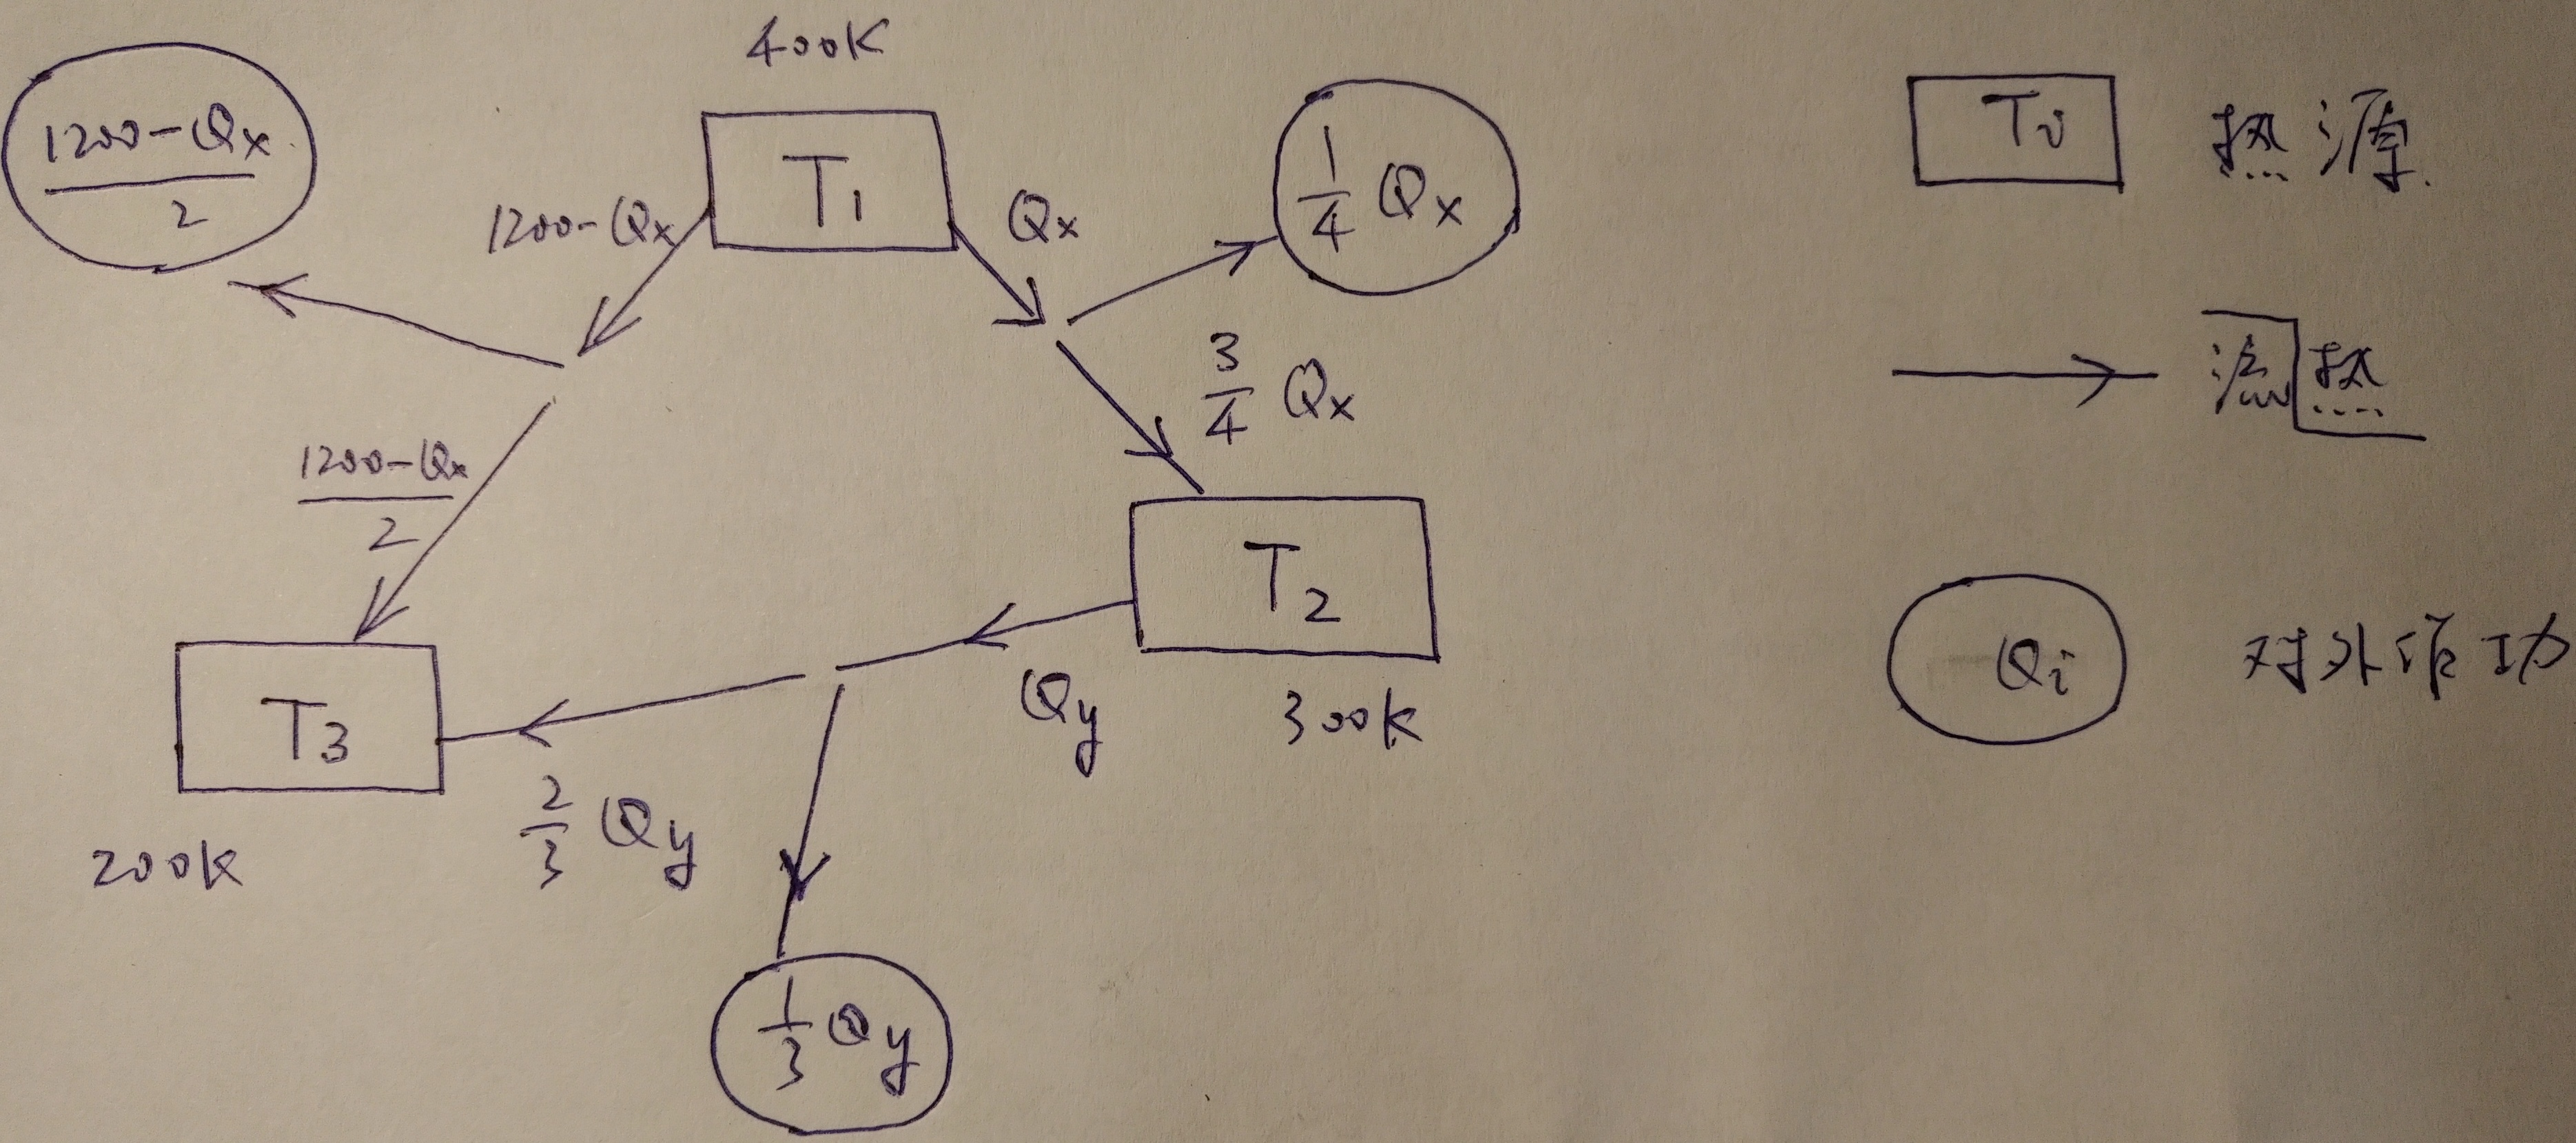
\includegraphics[width=0.5\textwidth]{heat-machine}
\end{figure}
由图, 我们有以下关系:
\begin{eqnarray*}
\frac{1200-Q_x}{2} + \frac{Q_y}{3} + \frac{Q_x}{4} = 200 & \Rightarrow & \frac{3}{4}Q_x - Q_y = 1200 \\
& \Rightarrow &
\begin{cases}
Q_2 = \frac{3}{4} Q_x - Q_y = 1200 J \\
Q_3 = \frac{1200-Q_x}{2} + \frac{2Q_y}{3} = -200 J
\end{cases} \\
& \Rightarrow & 
\begin{cases}
\Delta S_1 = \frac{Q_1}{T_1} = \frac{-1200}{400} = -3J/K \\
\Delta S_2 = \frac{Q_2}{T_2} = \frac{1200}{300} = 4J/K \\ 
\Delta S_3 = \frac{}{Q_3}{T_3} = \frac{-200}{200} = -1J/K \\
\Delta S_{\text{总}} = \sum_{i = 1}^{3} \Delta S_{i} = 0J/K.
\end{cases}
\end{eqnarray*}

\subsection{习题1.23}
考虑等熵过程($ S = S_{0} $), 
\begin{eqnarray*}
W_{S_{0}} = \int_{V_{0}}^{V} p(S_{0},V') \dd V' = RS_{0} \ln \frac{V}{V_{0}} & \Rightarrow & p(S_{0}, V) = \frac{\dd W_{S_{0}}}{\dd V} = \frac{RS_{0}}{V} \\
U(S_{0},V) - U(S_{0},V_{0}) = - W_{S_{0}} & \Rightarrow & U(S_{0},V) = U_{0} - RS_{0} \ln \frac{V}{V_{0}}.
\end{eqnarray*}
现在考虑一个等体过程($ V, S_{0} \rightarrow V, S $), 
\begin{align*}
U(S, V) - U(S_{0}, V) & = \int_{T(S_{0},V)}^{T(S,V)} T(S',V) \dd S' \\
& = \int_{S_{0}}^{S} \frac{RV_{0}}{V}\left( \frac{S'}{S_{0}} \right)^{a} \dd S' \\
& = \frac{RV_{0}S_{0}}{(a+1)V} \left[ \left( \frac{S}{S_{0}} \right)^{a+1} - 1 \right]
\end{align*}
因此,
\[ U(S, V) = \frac{RV_{0}S_{0}}{(a+1)V} \left[ \left( \frac{S}{S_{0}} \right)^{a+1} - 1 \right] - RS_{0} \ln \frac{V}{V_{0}} + U_{0} \]
又由: 
\[ \left( \frac{\partial p}{\partial S} \right)_{V} = - \left( \frac{\partial T}{\partial V} \right)_{S} = \frac{RV_{0}}{V^2} \left( \frac{S}{S_{0}} \right)^a \]
\[ \Rightarrow \quad{} p(S,V) = \frac{RV_{0}S_{0}}{(a+1)V^2} \left[ \left( \frac{S}{S_{0}} \right)^{a+1} - 1 \right] + \frac{RS_{0}}{V} \]
\[ W(S, V_{0} \rightarrow V) = \int_{V_{0}}^{V} p(S,V') \dd V' = 
\frac{RV_{0}S_{0}}{a+1} \left[ \left( \frac{S}{S_{0}} \right)^{a+1} - 1 \right] \left( \frac{1}{V_{0}} - \frac{1}{V} \right) + RS_{0} \ln \frac{V}{V_{0}}. \]


\end{document}